% Schematic representation of mach zender interferometer
% Modified from a version created by Henrik Kröger, https://github.com/derhedwig/fiberoptics/blob/master/auswertung.tex
% Author: Orlando Torres (2016)

\documentclass{standalone}
\usepackage{amsmath} % Required for \varPsi below
\usepackage{tikz,pgfplots}
\usetikzlibrary{calc}
\usetikzlibrary{patterns}

\begin{document}
  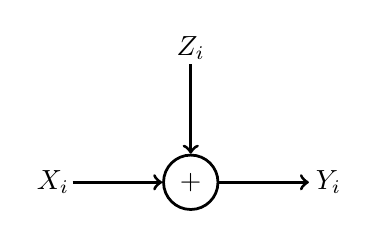
\begin{tikzpicture}
   	%define colors
    \definecolor{bbblue}{rgb}{0.964, 0.866, 0.474}
    \definecolor{rrred}{rgb}{0.952, 0.815, 0.105}
    \definecolor{yyyellow}{rgb}{0.925, 0.827, 0.152}    
    %0.933, 0.756, 0.227
    \definecolor{lblue}{rgb}{0.352, 0.556, 0.886}
    \definecolor{sblue}{rgb}{0.607, 0.733, 0.929}
	\definecolor{lyel}{rgb}{0.925, 0.827, 0.152}
    
    %define coordinates for modulator (upper side)
    \coordinate (in) at (-15.0mm, 0);
    \coordinate (out) at (15.0mm, 0);
	\coordinate (in2) at (0, 15mm);
	\coordinate (ce) at (0, 0);
    
    % Substrate, modulators, Waveguides, MMI and converters %
    
    \node [shape=circle, minimum width=5mm, minimum height=5mm, line width=0.35mm, color=black, draw]
    (ce) at (0,0) {+}; 

   
	\draw [->,line width=0.40mm, color=black]  (in) -- (ce);
	\node [align=left] (in) at ($(in) - (2.5mm, 0mm)$) {$X_i$};
	\draw [->,line width=0.40mm, color=black]  (ce) -- (out);
	\node [align=left] (in) at ($(out) + (2.5mm, 0mm)$) {$Y_i$};
	\draw [->,line width=0.40mm, color=black]  (in2) -- (ce);
	\node [align=left] (in) at ($(in2) + (0mm, 2mm)$) {$Z_i$};
    
  \end{tikzpicture}
\end{document}